\subsection{Wyniki dla podziału na $m$ obszarów}

Ten podrozdział opisuje wyniki podziału siatki podzielonej na $m \cdot k$ partycji na $m$ partycji, z których każda
zawiera $k$ podobszarów.
Dla tej części zakładam, że podział na $m \cdot k$ partycji jest na równe, bądź niemal równe części i podaję
wyniki tylko dla podziału na $m$ partycji po $k$ podobszarów każda.

Różnica w postacji wywołania algorytmu dla tej części polega na tym, że wykonywanych jest $100$ iteracji
partycjonowania na $m \cdot k$ partycji, a dla każ∂ego z tych podziałów wykonywanie jest $100$ iteracji poszukiwania
najlepszego podzielenia tych $m \cdot k$ partycji na $m$ partycji po $k$ podobszarów każda.
Jest to możliwe, ponieważ szukanie $m$ ma niski koszt obliczeniowy.
Ze wszystkich wywołań wybierane jest ten podział na $m$ partycji, który ma najkrótszą długość granic.
Długość granic pod rysunkiem podawana jest dla podziału na $m$ obszarów.

\begin{figure}[h]
\centering
\begin{subfigure}{.33\textwidth}
    \centering
    \fbox{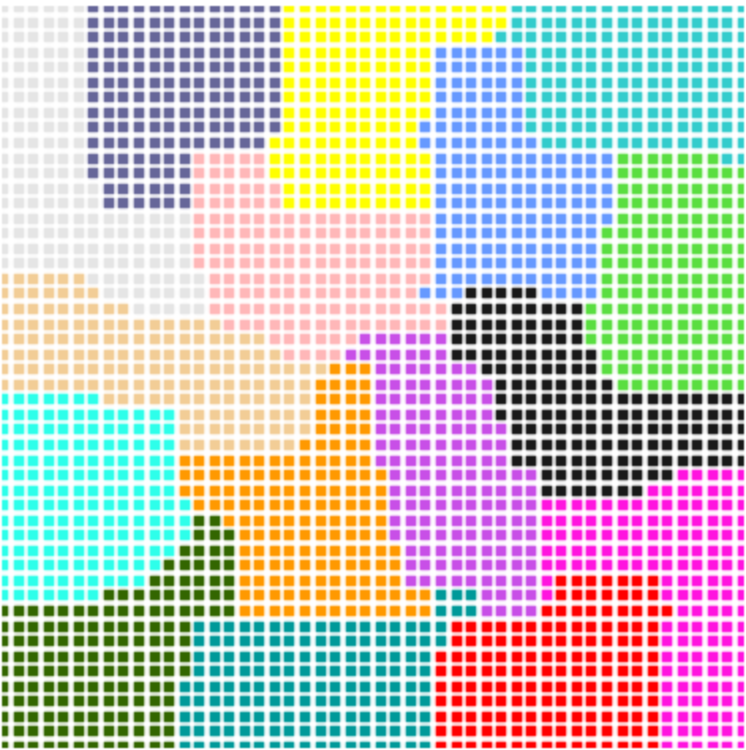
\includegraphics[width=0.7\linewidth]{images/results/m/1/mk}}
    \caption[short]{}
\end{subfigure}%
\begin{subfigure}{.33\textwidth}
    \centering
    \fbox{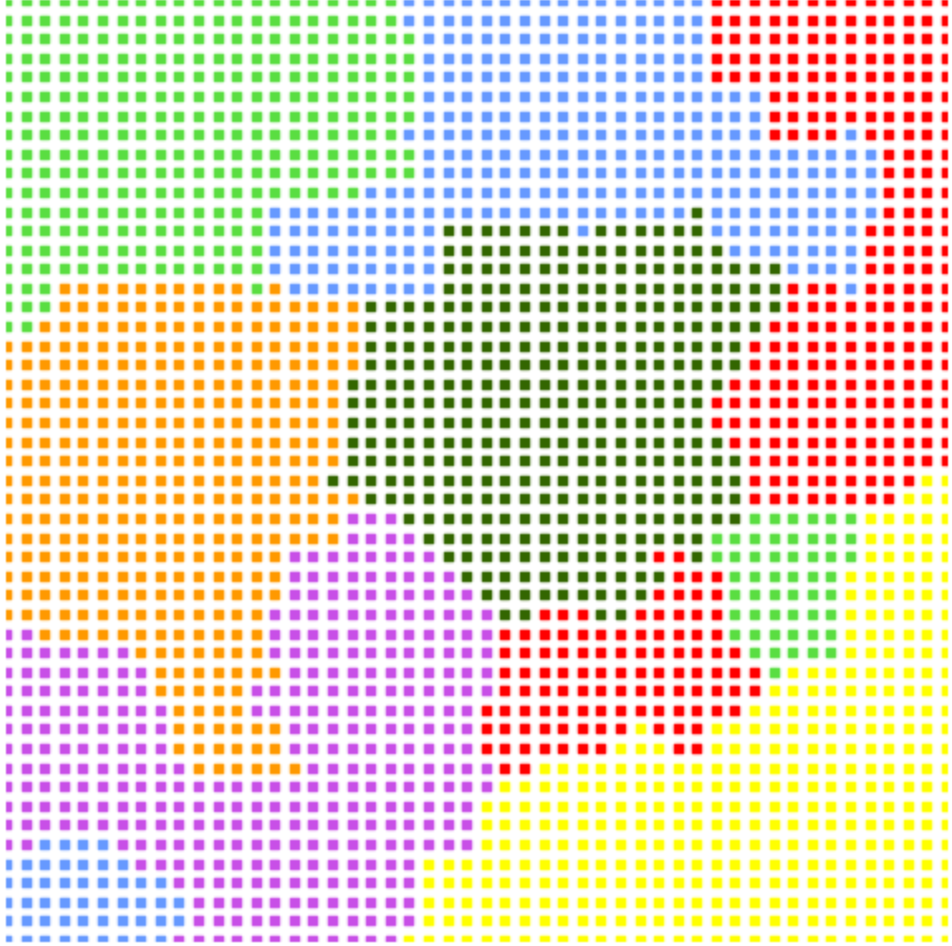
\includegraphics[width=0.7\linewidth]{images/results/m/1/m}}
    \caption[short]{}
\end{subfigure}%
\begin{subfigure}{.33\textwidth}
    \centering
    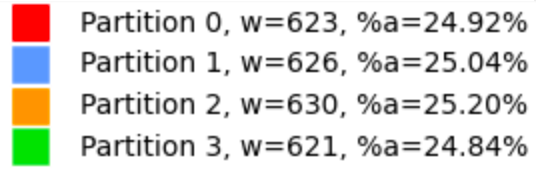
\includegraphics[width=0.9\linewidth]{images/results/m/1/results}
    \caption[short]{}
\end{subfigure}
\caption{Siatka $100$x$100$. Podział na $16$ partycji.
Obszary wyłączone z obliczeń nie są mapowane na wierzchołki.
Sumaryczna długość granic dla tego wyniku wynosi $382$.
Wybór najlepszego rezultatu wedle kryterium najmniejszej długości granic.}
\label{result:m:1}
\end{figure}